\documentclass[11pt]{article}
\usepackage{url}
\usepackage{latexsym,amssymb,amsmath,theorem,proof,calc,alltt}
%\usepackage{parsetree}
%\usepackage{tree-dvips}
\usepackage{pst-tree}
\usepackage{graphicx}
\DeclareGraphicsExtensions{.jpg}


%%%%%%%%%%%%%%%%%%%%%%%%%%%%%%%%%%%%
%                                  % 
%  VERSION Jan 2005                %
%                                  %
%%%%%%%%%%%%%%%%%%%%%%%%%%%%%%%%%%%%

\newtheorem{theorem}{Theorem}
\newtheorem{definition}[theorem]{Definition}
\newtheorem{proposition}[theorem]{Proposition}
\newtheorem{fact}[theorem]{Fact}
\newtheorem{lemma}[theorem]{Lemma}
\newtheorem{corollary}[theorem]{Corollary}
\newtheorem{question}[theorem]{Question}
\newtheorem{claim}[theorem]{Claim}
\newtheorem{observation}[theorem]{Observation}

\newenvironment{proof}{\noindent \bf Proof. \  \rm}{\hfill $\Box$}

\newtheorem{condition}{Condition}[section]
\newtheorem{nl}{}

\newtheorem{axiom}{A}
\newtheorem{erax}{A$^{\mbox{\bf e}}$}
\newtheorem{erth}{T$^{\mbox{\bf e}}$}
\newtheorem{theo}{T}
\newtheorem{defi}{D}
\newtheorem{derrule}{R}

\newenvironment{digression}{{\bf Digression\ }}{{\bf End of digression.}}
\newenvironment{prf}{{\bf Proof:\ }}{\hspace*{\fill}\rule{1 ex}{1 ex}}

%\newcommand{\proof}{{\bf Proof:\ }} 
\newcommand{\theend}{\hspace*{\fill}\rule{1 ex}{1 ex} \\[2ex]}
\newcommand{\vtheend}{\hspace*{\fill}\rule{1 ex}{1 ex}}
%\newcommand{\proofend}{\hspace*{\fill}\rule{1 ex}{1 ex}}
\newcommand{\commentout}[1]{}
\newcommand{\handout}[1]{\#}

\newcommand{\conc}{\hat{\ }}

\newcommand{\impl}{\rightarrow}
\newcommand{\simpl}{\Rightarrow}
\newcommand{\mequiv}{\leftrightarrow}
\newcommand{\sequiv}{\Leftrightarrow}
\newcommand{\weakneg}{\mbox{$\sim$}}
\newcommand{\undef}{\uparrow}

\newcommand{\UnivCl}{\mbox{$\forall\!\!\!\forall$}}

\newcommand{\VE}{\mbox{\em VE}}
\newcommand{\NF}{\mbox{\em NF}}
\newcommand{\nf}{n\!f}

\newcommand{\dotminus}{\dot{-}}
\newcommand{\eqdef}{\stackrel{\rm def}{\iff}}
\newcommand{\isdef}{\stackrel{\rm def}{=}}

\newcommand{\pow}{{\cal P}}
%{\mbox{\large\wp}}
\newcommand{\dom}{{\rm dom\:}}
\renewcommand{\int}{{\rm int\:}}
\newcommand{\rng}{{\rm rng\:}}
\newcommand{\tick}{\surd}

\newcommand{\tto}{{\to\!\!\!\!\to}}


%\newcommand{\0}{{\bf 0}}
%\newcommand{\1}{{\bf 1}}
\newcommand{\2}{{\bf 2}}
\newcommand{\3}{{\bf 3}}
\newcommand{\4}{{\bf 4}}
\newcommand{\5}{{\bf 5}}
\newcommand{\Ln}{{\cal L}}
\newcommand{\Lnq}{{\cal L}_{\cal Q}}
\newcommand{\cA}{{\cal A}}
\newcommand{\M}{{\cal M}}
\newcommand{\K}{{\cal K}}
\newcommand{\I}{{\cal I}}
\newcommand{\N}{{\cal N}}
\newcommand{\Q}{{\bf Q}}
\newcommand{\W}{{\bf W}}
\newcommand{\cQ}{{\cal Q}}
\newcommand{\cS}{{\cal S}}
\newcommand{\dQ}{\dot{{\bf Q}}}
\newcommand{\T}{{\bf T}}
\newcommand{\A}{{\bf A}}
\newcommand{\B}{{\bf B}}
\newcommand{\C}{{\bf C}}

\newcommand{\bfa}{\mbox{\bf a}}
\newcommand{\bfb}{\mbox{\bf b}}
\newcommand{\bfc}{\mbox{\bf c}}
\newcommand{\bfd}{\mbox{\bf d}}
\newcommand{\bfe}{\mbox{\bf e}}
\newcommand{\bff}{\mbox{\bf f}}
\newcommand{\bfg}{\mbox{\bf g}}
\newcommand{\bfh}{\mbox{\bf h}}
\newcommand{\bfi}{\mbox{\bf i}}
\newcommand{\bfj}{\mbox{\bf j}}

\newcommand{\bfx}{\mbox{\bf x}}
\newcommand{\bfy}{\mbox{\bf y}}
\newcommand{\bfz}{\mbox{\bf z}}

\newcommand{\ldbrack}{\lbrack\!\lbrack}
\newcommand{\ldb}{\lbrack\!\lbrack}
\newcommand{\rdbrack}{\rbrack\!\rbrack}
\newcommand{\rdb}{\rbrack\!\rbrack}
\newcommand{\negmod}{\mbox{$\:=\!\!\!|\,$}}
\newcommand{\notnegmod}{\mbox{$\:\neq\!\!\!|\,$}}

\newcommand{\mi}[1]{\mbox{\it #1}}
\newcommand{\mb}[1]{\mbox{\bf #1}}
\newcommand{\down}{\mbox{$\downarrow$}}
\newcommand{\forces}{\mbox{\ $\vdash\!\!\!\vdash$\ }}
\newcommand{\negforces}{\mbox{\ $\dashv\!\!\!\dashv$\ }}
\newcommand{\notforces}{\mbox{\ $\vdash\!\!\!\not\vdash$\ }}
\newcommand{\notnegforces}{\mbox{\ $\dashv\!\!\!\not\dashv$\ }}
\newcommand{\bom}[1]{\mbox{\boldmath $#1$}}
\newcommand{\bme}[1]{\mbox{\boldmath $\LA #1 \RA$}}
\newcommand{\bmu}[1]{\mbox{\boldmath $[ #1 ]$}}
\newcommand{\bmeu}[1]{\mbox{\boldmath $( #1 )$}}

\renewcommand{\phi}{\varphi}

\newcommand{\ba}{\begin{eqnarray}}
\newcommand{\ea}{\end{eqnarray}}
%\newcommand{\ex}[1]{&&\mbox{\em{}#1}}
%\newcommand{\exnn}[1]{&&\mbox{\em{}#1} \nonumber}
%\newcommand{\form}[1]{&&\mbox{\em{}}#1}
%\newcommand{\formnn}[1]{&&\mbox{\em{}}#1 \nonumber}
\newcommand{\sepline}{\cline{3-3}}
\newcommand{\sref}[1]{(\ref{#1})}

\newcommand{\NI}{\noindent}
\newcommand{\VV}{\vspace{2 ex}}

\newcommand{\LA}{\langle}
\newcommand{\RA}{\rangle}


% for letters 

\newcommand{\addressee}[1]{%
{\qquad\qquad\qquad\qquad\qquad\qquad\qquad\qquad\qquad\parbox{10in}
% name and address of adressee
{#1}}
}


\newcommand{\close}[1]{\begin{array}{c}{#1} \\ {\times} \end{array}}
\newcommand{\clsubs}[2]{\begin{array}{c}{#1} \\ {#2} \end{array}}
\newcommand{\stack}[1]{\begin{array}{c}{#1} \end{array}}
\newcommand{\barr}{\begin{array}{c}}
\newcommand{\earr}{\end{array}}

\newcommand{\EQ}{\approx}
\newcommand{\NEQ}{\not\approx}

\newcommand{\var}{{\rm var\:}}
%\newcommand{\dom}{{\rm dom\:}}
%\newcommand{\rng}{{\rm rng\:}}

\newcommand{\bB}{\mbox{\boldmath $B$}}

\newcommand{\ttop}{\mbox{\boldmath $\top\!\!\!\!\top$}}
\newcommand{\bbot}{\mbox{\boldmath $\bot\!\!\!\!\bot$}}

\newcommand{\bT}{\mbox{\boldmath $T$}}
\newcommand{\cB}{\mbox{$\cal B$}}

\newcommand{\cE}{{\cal E}}

\newcommand{\href}[1]{}
\newcommand{\Nat}{\mathbb{N}}
\newcommand{\Exists}{\boldsymbol{\exists\!\!\!\exists}}
\newcommand{\Forall}{\boldsymbol{\forall\!\!\!\forall}}
\newcommand{\Neg}{\boldsymbol{\neg\!\!\!\neg}}
\newcommand{\SC}{\ \boldsymbol{;}\ }

\newsavebox{\fminibox}
\newlength{\fminilength}
\newenvironment{fminipage}[1][\linewidth]
 {\setlength{\fminilength}{#1-2\fboxsep-2\fboxrule-1em}%
  \bigskip\begin{lrbox}{\fminibox}\quad\begin{minipage}{\fminilength}\bigskip}
 {\smallskip\end{minipage}\end{lrbox}\noindent\fbox{\usebox{\fminibox}}\bigskip}

\newcommand{\bc}{\begin{fminipage}}
\newcommand{\ec}{\end{fminipage}}

\newenvironment{code}{\begin{fminipage}\begin{alltt}}%
{\end{alltt}\end{fminipage}}

\newenvironment{pcode}{\begin{fminipage}\begin{alltt}}%
{\end{alltt}\end{fminipage}
}

\renewcommand{\impl}{\Rightarrow}

\newtheorem{exercise}[theorem]{Exercise}

\newcommand{\produces}{\longrightarrow}
\newcommand{\yields}{\Rightarrow}

\setlength{\textheight}{22cm}
\setlength{\textwidth}{16cm}
\setlength{\topmargin}{0cm}
\setlength{\oddsidemargin}{0cm}
\setlength{\evensidemargin}{0cm}

\setlength{\parindent}{0 ex} 
\setlength{\parskip}{1.5 ex}

\newcommand{\Ibox}[1]{[{\scriptstyle\:#1\: }]}
\newcommand{\Idia}[1]{\langle{\scriptstyle\: #1\: }\rangle}
\newcommand{\Icbox}[1]{[{\scriptstyle\: #1\:}]^{\:\breve{}}}
\newcommand{\Icdia}[1]{\langle{\scriptstyle\: #1\: }\rangle^{\breve{}}}
\newcommand{\Cbox}{\Box^{\:\breve{}}}
\newcommand{\Cnu}{\nu^{\:\breve{}}}
\newcommand{\Cdia}{\Diamond^{\breve{}}}
\newcommand{\Cpi}{\pi^{\breve{}}}


\title{Relational Analysis of Software Systems} 

\author{Jan van Eijck\thanks{CWI, Amsterdam
        and Uil-OTS, Utrecht, \texttt{jve@cwi.nl}}, 
        Paul Klint\thanks{CWI, Amsterdam
        and Informatics Institute, University of Amsterdam, \texttt{paulk@cwi.nl}}
        and 
        Tijs van der Storm\thanks{CWI, Amsterdam,\texttt{storm@cwi.nl}}
}

\begin{document}

\maketitle 

\begin{abstract} \noindent
We present relational tools for analysing (large) software systems,
based on an appropriate Haskell datatype for relations derived from
Chapter 5 of \cite{DoeEij04:thr}. The main purpose is to demonstrate
some very concrete applications of abstract relations, and to develop 
a relational analysis tool for software engineering in an appropriate 
functional language. Our tool is written in Haskell 98
\cite{Haskell98:rep}, in `literate programming' style \cite{Knuth:lp}.
\end{abstract} 

\paragraph{Keywords:} \ldots

%\paragraph{MSC codes:} 03B10, 03F03, 68N17, 68T15 

\section{Introduction} 

To be written

\section{Module Declaration} 

\bc\begin{verbatim}
module RASS ( 

        module Set,
        module Graph,
        module GraphViz,
        module RASS

) where 

import List
import System.IO.Unsafe (unsafePerformIO) 
import Char
import Set
import Graph
import GraphViz
\end{verbatim}\ec

The modules \verb^List^,  \verb^System^, \verb^System.IO.Unsafe^, \verb^Char^, 
are standard Haskell modules, for operations on lists and characters, 
for input/output routines, and for input/output outside the IO monad (`unsafe IO'), 
respectively. The three modules \verb^Set^, \verb^Graph^ 
and \verb^GraphViz^ are given in the appendices below. 


%The module
%\verb^ATermLib^ is the Haskell Aterm library that is 
%part of {\em Strafunski}, a Haskell software bundle for 
%generic programming and language processing \cite{LaeVis03:asal}. 
%Aterms or `annotated terms' are documented in \cite{BraJonKli00:eat}.

\section{Analyzing Procedure Call Structure}

This example is from \cite{Klint03:atitr}. 

Declaring types for procedure names and component names:

\bc\begin{verbatim} 
type Procedure = String
type Component = String 
\end{verbatim}\ec

An example of a procedure calling relation (the links indicate 
direct calls). 

\bc\begin{verbatim}
calls :: Rel Procedure
calls = makeR [("a","b"),("b","c"),("b","d"),("d","c"),("d","e"),
               ("f","e"),("f","g"),("g","e")]
\end{verbatim}\ec

The relation displayed as it is encoded: 

\begin{verbatim}
RASS> calls
({"a","b","c","d","e","f","g"},
 {"a","b","c","d","e","f","g"},
  array (0,6) [(0,{1}),(1,{2,3}),(2,{}),(3,{2,4}),(4,{}),(5,{4,6}),(6,{4})])
\end{verbatim}

The set of edges of the relation: 

\begin{verbatim}
RASS> edges calls
{("a","b"),("b","c"),("b","d"),("d","c"),("d","e"),("f","e"),("f","g"),("g","e")}
\end{verbatim}

Graphical display via the {\em dot} \cite{KouNor:dgwd}
visualisation tool (\verb^writeRel^ writes the source for  {\em dot}
to a file): 

\begin{verbatim}
RASS> writeRel "calls" calls
\end{verbatim} 

The result: 

\begin{center}
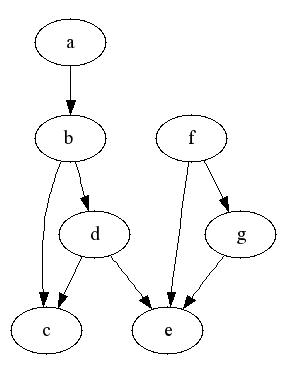
\includegraphics[width=2.5in]{calls}
\end{center}

\paragraph{Number of procedure calls} 

\begin{verbatim} 
RASS> size (edges calls)
8
\end{verbatim}

\paragraph{Number of procedures} 

\begin{verbatim} 
RASS> size (carrier calls)
7
\end{verbatim}

\paragraph{Entry points (or sources)} 

\begin{verbatim} 
RASS> sources calls
{"a","f"}
\end{verbatim} 

\paragraph{Leaves (or sinks)} 

\begin{verbatim} 
RASS> sinks calls
{"c","e"}
\end{verbatim} 

\paragraph{Indirect calls} 

\begin{verbatim}
RASS> edges (tc calls)
{("a","b"),("a","c"),("a","d"),("a","e"),("b","c"),("b","d"),("b","e"),
("d","c"),("d","e"),("f","e"),("f","g"),("g","e")}
\end{verbatim}

Viewed as a graph: 

\begin{center}
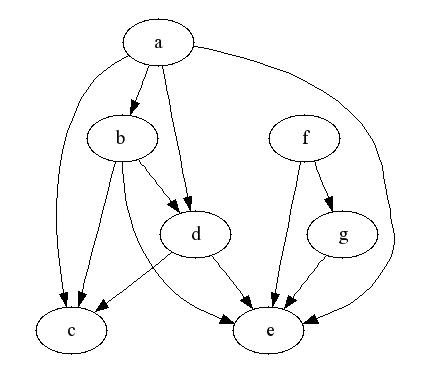
\includegraphics[width=3in]{tcalls}
\end{center}


\paragraph{Calls from given entry points} 

\begin{verbatim}
RASS> rightSection (tc calls) "a"
{"b","c","d","e"}
RASS> rightSection (tc calls) "f"
{"e","g"}
\end{verbatim}

\paragraph{Procedures called from all entry points} \mbox{}

\begin{verbatim}
RASS> commonDescendants calls (sources calls)
{"e"}
\end{verbatim}

\section{Analyzing the Component Structure of an Application} 

The following example is again from \cite{Klint03:atitr}.
Suppose the following relation gives the direct procedure dependencies of 
an application: 

\bc\begin{verbatim}
calls2 :: Rel Procedure 
calls2 = makeR [("main","a"),("main","b"),("a","b"),
                ("a","c"),("a","d"),("b","d")]
\end{verbatim}\ec

In graph format: 

\begin{center}
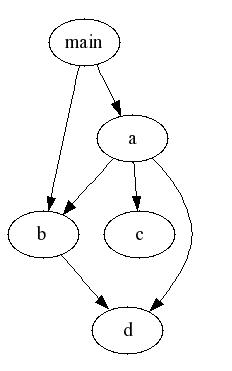
\includegraphics[width=2in]{calls2}
\end{center}

Suppose the mapping from procedures to the components to which they belong is 
as follows: 

\bc\begin{verbatim} 
belongsTo :: Procedure -> Component 
belongsTo "main" = "Appl"
belongsTo "a"    = "Appl"
belongsTo "b"    = "DB"
belongsTo "c"    = "Lib"
belongsTo "d"    = "Lib"
\end{verbatim}\ec

Then the dependency structure between procedures can be lifted to a 
dependency structure between components by means of the following function: 

\bc\begin{verbatim}
lift :: (Ord a, Ord b) => (a -> b) -> Rel a -> Rel b
lift f = makeR . (map (\ (x,y) -> (f x, f y))) . edgelist
\end{verbatim}\ec 

We get:

\begin{verbatim} 
RASS> edges (lift belongsTo calls2)
{("Appl","Appl"),("Appl","DB"),("Appl","Lib"),("DB","Lib")}
RASS> writeRel "components" (lift belongsTo calls2)
\end{verbatim}

The \verb^components^ file displayed in graph format: 

\begin{center}
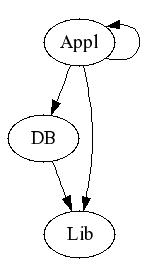
\includegraphics[width=1.5in]{components}
\end{center}

\section{Dataflow} 

The following examples,  based on Aho, Sethi and Ullman 
\cite{AhoSetUll:cptt}, 
concern flow of control in computations. Nodes in a flow graph
represent computations in basic blocks (where the computation 
starts at the beginning of the block and leaves at the end, without
halt or possibility of branching except at the end), 
edges represent the flow of control between basic blocks. 
An edge from block $B_1$ to block $B_2$ expresses that $B_2$ can 
immediately follow $B_1$ in some execution sequence. 

Here is an example flow graph taken from \cite{AhoSetUll:cptt}.

\bc\begin{verbatim}
flow :: Rel Int
flow = makeR [(1,2),(1,3),(2,3),(3,4),(4,3),(4,5),(4,6),(5,7),(6,7),
              (7,4),(7,8),(8,9),(8,10),(8,3),(9,1),(10,7)]
\end{verbatim}\ec

Viewed as a graph: 

\begin{center}
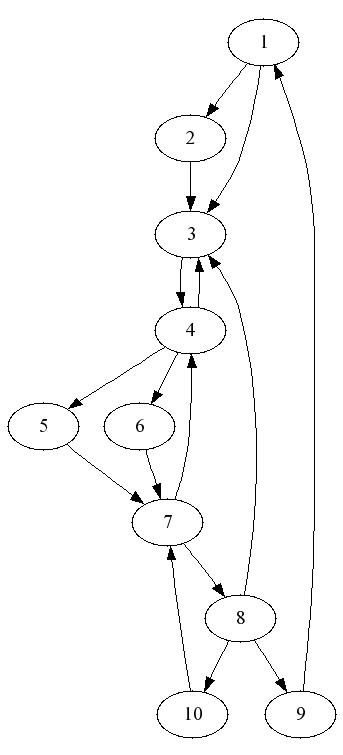
\includegraphics[width=2.5in]{flow}
\end{center}

\paragraph{Domination} \mbox{}


\cite{AhoSetUll:cptt}, Section 10.4, defines the relation of domination on 
flow graphs as follows. 
\begin{quote}
 Let a flow graph $G$ and an initial node $i$ in the graph be given. \\
 $d$ dominates $n$ in $(G,i)$ if every path from $i$ to $n$ passes through $d$. 
\end{quote}

Aho, Sethi and Ullman note that the dominate relation is reflexive:
every node $n$ dominates itself, for every path from $i$ to $n$ ends
in $n$.

Note that the initial node has to be given explicitly. Taking the set
of initial nodes to be the sources of the relation will not work (the
example graph has no sources).

The importance of the domination relation is in loop detection. See below. 

Here is a straightforward implementation of the definition:

\bc\begin{verbatim} 
domi  :: Ord a => Rel a -> a -> Rel a
domi r i = 
  let  
    univ = edgelist (total (carrier r))
   in 
     makeR [ (d,n) | (d,n) <- univ, 
                      not (inSet n (avoidFrom r i d)) ]
\end{verbatim}\ec

This gives: 

\begin{verbatim}
RASS> edges (domi flow 1)
{(1,1),(1,2),(1,3),(1,4),(1,5),(1,6),(1,7),(1,8),(1,9),(1,10),
 (2,2),(3,3),(3,4),(3,5),(3,6),(3,7),(3,8),(3,9),(3,10),(4,4),
 (4,5),(4,6),(4,7),(4,8),(4,9),(4,10),(5,5),(6,6),(7,7),(7,8),
 (7,9),(7,10),(8,8),(8,9),(8,10),(9,9),(10,10)}
\end{verbatim}

Write the source for {\em dot}\/: 

\begin{verbatim}
RASS> writeRel "domi" (domi flow 1)
\end{verbatim} 

The result displayed: 

\begin{center}
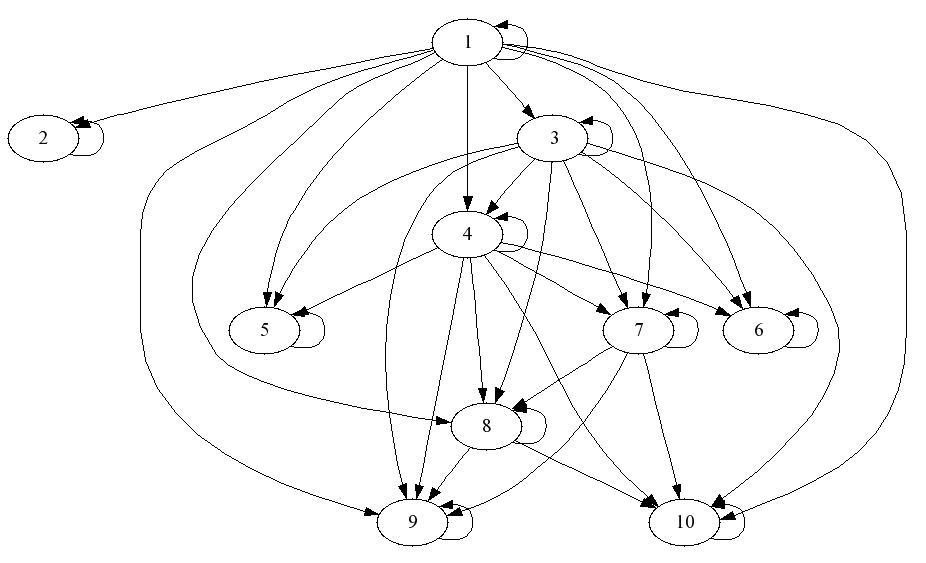
\includegraphics[width=5in]{domi}
\end{center}

Aho, Sethi and Ullman define immediate dominators in terms of
domination, as follows.

\begin{quote} 
 Let a flow graph $G$ and an initial node $i$ in the graph be given. \\
 $m$ immediately dominates $n$ in $(G,i)$ if 
  \begin{itemize}   
    \item $m$ dominates $n$ in $(G,i)$, 
    \item if $d \neq n$ and $d$ dominates $n$ in $(G,i)$, 
          then $d$ dominates $m$ in $(G,i)$. 
  \end{itemize} 
\end{quote}

This definition has a flaw, for it omits the crucial condition 
of irreflexivity. We amend it as follows: 

\begin{quote} 
 Let a flow graph $G$ and an initial node $i$ in the graph be given. \\
 $m$ immediately dominates $n$ in $(G,i)$ if 
  \begin{itemize}   
    \item $m$ dominates $n$ in $(G,i)$, 
    \item $m \neq n$, 
    \item if $d \neq n$ and $d$ dominates $n$ in $(G,i)$, 
          then $d$ dominates $m$ in $(G,i)$. 
  \end{itemize} 
\end{quote}

Here is the implementation (again, we can follow the definition to the
letter):

\bc\begin{verbatim}
idomi :: Ord a => Rel a -> a -> Rel a 
idomi r i = 
  let
    dr = domi r i
  in 
  makeRL 
   [ (m,n) | (m,n) <- edgelist dr,
              m /= n, 
              all (\ k -> inSet k (leftSection dr m))
                  [ d | (d,e) <- edgelist dr, e == n, d /= n ]   ]
\end{verbatim}\ec

This gives: 

\begin{verbatim} 
RASS> edges (idomi flow 1)
{(1,2),(1,3),(3,4),(4,5),(4,6),(4,7),(7,8),(8,9),(8,10)}
\end{verbatim}

Write the source for {\em dot}\/: 

\begin{verbatim}
RASS> writeRel "idom" (idomi flow 1)
\end{verbatim} 

The result displayed: 

\begin{center}
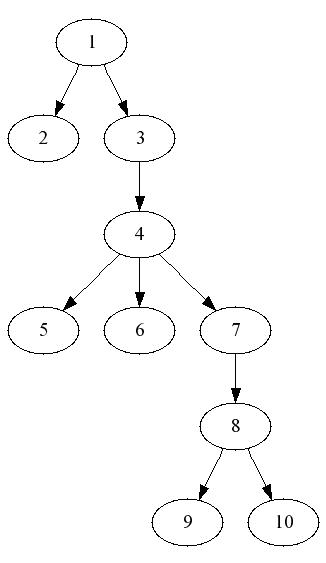
\includegraphics[width=2.5in]{idom}
\end{center}

This is what Aho, Sethi and Ullman call the dominator tree for the flow graph. 

\paragraph{Loop Detection}  \mbox{}

Informally, a loop in a flow graph is a set of strongly connected nodes in 
the graph with a single entry point. 

Loops in a graph can be found by searching for {\em back edges}, edges $(n,m)$ 
in the graph with the property that $m$ dominates $n$. Here is the implementation: 

\bc\begin{verbatim} 
backedges :: Ord a => Rel a -> a -> [(a,a)]
backedges r i = [ (n,m) | (n,m) <- edgelist r, 
                          elem (m,n) (edgelist (domi r i) ) ]
\end{verbatim}\ec

This gives: 

\begin{verbatim}
RASS> backedges flow 1
[(4,3),(7,4),(8,3),(9,1),(10,7)]
\end{verbatim}

These are indeed the edges through which the flow graph loops. 

Next, we define the natural loops. The natural loop of back edge $(n,m)$ 
is the set that contains $m$ together with all nodes that can reach $n$ while 
avoiding $m$: 

\bc\begin{verbatim} 
naturalLoop :: Ord a => Rel a -> a -> (a,a) -> Set a
naturalLoop r i (n,m) = insertSet m (avoidTo r n m)
\end{verbatim}\ec

The natural loops of a given flow graph: 

\bc\begin{verbatim}
naturalLoops :: Ord a => Rel a -> a -> [Set a]
naturalLoops r i = map (naturalLoop r i) (backedges r i)
\end{verbatim}\ec

Applied to the example, we get: 

\begin{verbatim}
RASS> naturalLoops flow 1
[{3,4,5,6,7,8,10},{4,5,6,7,8,10},{3,4,5,6,7,8,10},{1,2,3,4,5,6,7,8,9,10},
 {7,8,10}]
\end{verbatim}

Note that backedges to the same node yield the same natural loop: 
$(4,3)$ and $(8,3)$ both yield the loop $\{3,4,5,6,7,8,10\}$. 

\section{Representing Program Fragments as Areas} 

An \verb^Area^ is a triple consisting of a file name and two pairs, 
where the first pair gives a begin line and a begin column in the file, 
and the second pair an end line and an end column. 

\bc\begin{verbatim}
data Area = Area String (Int,Int) (Int,Int) deriving (Eq,Ord,Read)
\end{verbatim}\ec

Showing areas: 

\bc\begin{verbatim} 
instance Show Area where 
  show (Area name begin end) = name ++ show begin ++ show end
\end{verbatim}\ec

Converting from a quintuple to an area: 

\bc\begin{verbatim}
toArea :: (String, Int, Int, Int, Int) -> Area
toArea (name, l1, p1, l2, p2) 
   | l1 > l2             = error "end line before begin line"
   | l1 == l2 && p1 > p2 = error "end pos before begin pos"
   | otherwise           = Area name (l1,p1) (l2,p2)
\end{verbatim}\ec

The relations \verb^part^ (being textually part of) 
and \verb^properPart^ (being textually strictly part of). 
Note that the first of these is a partial order, the second a 
strict partial order. The type of areas is {\em not} linearly ordered
by textual inclusion! 

\bc\begin{verbatim} 
part :: Area -> Area -> Bool
part (Area name1 begin1 end1) (Area name2 begin2 end2) = 
  name1 == name2 && begin2 <= begin1 && end1 <= end2

properPart :: Area -> Area -> Bool
properPart (Area name1 begin1 end1) (Area name2 begin2 end2) = 
  name1 == name2 && 
  or [begin1 == begin2 && end1 < end2, 
      begin1 > begin2  && end1 < end2, 
      begin1 > begin2  && end1 < end2]
\end{verbatim}\ec

\section{Relation input}

Make a file of Haskell definitions into a module: 

\bc\begin{verbatim} 
makeMod :: FilePath -> IO ()
makeMod name = do prefix <- return $ "module A where \n\nimport RASS\n\n"
                  str    <- readFile fname
                  writeFile mname (prefix ++ str)
  where fname = name ++ ".hs"
        mname = name ++ "MOD.hs"
\end{verbatim}\ec

\bc\begin{verbatim}
str2rl :: (Ord a, Read a, Ord b, Read b) => String -> Rl a b 
str2rl str = makeRL (read str)
\end{verbatim}\ec

Reading a relation (list of pairs, in Haskell format) from a file: 

\bc\begin{verbatim}
readRlFile :: (Ord a, Read a, Ord b, Read b) => FilePath -> Rl a b
readRlFile name = unsafePerformIO (do str <- readFile name 
                                      return (str2rl str))
\end{verbatim}\ec

Converting a string to a relation, assuming the types of the 
two argument places are the same: 

\bc\begin{verbatim}
str2rel :: (Ord a, Read a) => String -> Rel a
str2rel str = makeR (read str)
\end{verbatim}\ec

Reading a relation (list of pairs, in Haskell format) from a file,
assuming the types of the first and second elements of the pairs are
the same:

\bc\begin{verbatim}
readRelFile :: (Ord a, Read a) => FilePath -> Rel a
readRelFile name = unsafePerformIO (do str <- readFile name
                                       return (str2rel str))
\end{verbatim}\ec

\section{Relation Output} 

Define the class of showable types: 

\bc\begin{verbatim}
class ShowT a
 where
  showT :: a -> String
\end{verbatim}\ec

\bc\begin{verbatim} 
instance ShowT Int
 where
  showT _ = "Int"

instance ShowT String
 where
  showT _ = "String"

instance ShowT Area
 where 
  showT _ = "Area"

instance (ShowT a, ShowT b) => ShowT (a,b)
 where
  showT (a,b) = "(" ++ showT a ++ "," ++ showT b ++ ")"

instance ShowT a => ShowT [a]
 where
  showT l = "[" ++ showT (head l) ++ "]"
\end{verbatim}\ec

Convering a string to a correct function name: 

\bc\begin{verbatim} 
low :: String -> String 
low s = case span isAlphaNum s of 
   (x:xs,[]) -> if isAlpha x 
                  then (toLower x) : xs
                  else error  "incorrect name"
   _         -> error  "incorrect name"
\end{verbatim}\ec

Writing a relation to a file. 

\bc\begin{verbatim} 
wR ::  (Ord a, Show a, ShowT a, Ord b, Show b, ShowT b) => 
                                         String -> Rl a b -> IO()
wR name rel = 
  do typing <- return $ rname ++ " :: " ++ showT edges
     r      <- return $ typing ++ "\n" ++  rname ++ " = "  ++ show edges
     writeFile fname r
  where fname = name ++ ".hs"
        rname = low name 
        edges = edgelist rel
\end{verbatim}\ec

\section{Further Work} 

\begin{itemize} 

\item Interface to the ATerm library \cite{BraJonKli00:eat}. 

\item Interface to the Strafunski software bundle \cite{LaeVis03:asal}. 

\item Use RASS for realistic tasks. 

\item Performance comparison with Rscript \cite{Klint03:atitr}, \ldots 

\item If necessary for performance reasons: reimplement operations 
      on sets in terms of OBDDs. 

\item Update \cite{DoeEij04:thr} with motivating examples from 
      software engineering. 
\end{itemize} 

\paragraph{Acknowledgement} Thanks to Ralf L\"ammel for 
sound Haskell advice. 
    
\clearpage 
\appendix

\section{A Module for Sets}

This module is based on the software from \cite[Chapter 4]{DoeEij04:thr}.

\bc\begin{verbatim} 
module Set (Set(..),emptySet,isEmpty,inSet,subSet,insertSet,
            deleteSet,powerSet,power1Set,takeSet,(!!!),
            list2set,set2list,size,mapS,filterS,
            unionSet,intersectSet,diffSet, 
            genUnion)

where

import List (sort) 
\end{verbatim}\ec

We implement sets as ordered lists without duplicates, and 
show them in the usual set format $\{ a_1, a_2, \ldots \}$. 

\bc\begin{verbatim} 
newtype Set a = Set [a] deriving (Eq,Ord)

instance (Show a) => Show (Set a) where
    showsPrec _ (Set s) str = showSet s str

showSet []     str = showString "{}" str
showSet (x:xs) str = showChar '{' ( shows x ( showl xs str))
   where showl []     str = showChar '}' str
         showl (x:xs) str = showChar ',' (shows x (showl xs str))
\end{verbatim}\ec

The empty set: 

\bc\begin{verbatim} 
emptySet  :: Set a       
emptySet = Set []

isEmpty  :: Set a -> Bool            
isEmpty (Set []) = True
isEmpty _        = False
\end{verbatim}\ec

The `element of' ($\in$) relation: 

\bc\begin{verbatim}
inSet  :: (Ord a) => a -> Set a -> Bool  
inSet x (Set s) = elem x (takeWhile (<= x) s)
\end{verbatim}\ec

The `subset of' ($\subseteq$) relation: 

\bc\begin{verbatim}
subSet :: (Ord a) => Set a -> Set a -> Bool
subSet (Set []) _       = True  
subSet (Set (x:xs)) set = (inSet x set) && subSet (Set xs) set 
\end{verbatim}\ec

The operation of inserting an element into a set: 

\bc\begin{verbatim} 
insertSet :: (Ord a) => a -> Set a -> Set a 
insertSet x (Set s) = Set (insertList x s) 

insertList x [] = [x]
insertList x ys@(y:ys') = case compare x y of 
                                 GT -> y : insertList x ys' 
                                 EQ -> ys 
                                 _  -> x : ys 
\end{verbatim}\ec

Deleting an element from a set: 

\bc\begin{verbatim}
deleteSet :: Ord a => a -> Set a -> Set a 
deleteSet x (Set s) = Set (deleteList x s)

deleteList x [] = []
deleteList x ys@(y:ys') = case compare x y of 
                                 GT -> y : deleteList x ys'
                                 EQ -> ys'
                                 _  -> ys
\end{verbatim}\ec

Conversion from list to set: 

\bc\begin{verbatim}
list2set :: Ord a => [a] -> Set a
list2set xs = Set (foldr insertList [] xs)
\end{verbatim}\ec

Conversion from set to list: 

\bc\begin{verbatim}
set2list :: Set a -> [a] 
set2list (Set xs) = xs
\end{verbatim}\ec

Size of a set: 

\bc\begin{verbatim} 
size :: Set a -> Int
size = length . set2list
\end{verbatim}\ec

The $f$-map of a set $S$  is the set $\{ f x \mid x \in S \}$. 

\bc\begin{verbatim} 
mapS :: Ord b => (a -> b) -> Set a -> Set b
mapS f = list2set . map f . set2list
\end{verbatim}\ec

Filtering for sets: 

\bc\begin{verbatim} 
filterS :: Ord a => (a -> Bool) -> Set a -> Set a
filterS p = list2set . filter p . set2list
\end{verbatim}\ec

Implementation of power set $\pow A$: 

\bc\begin{verbatim}
powerSet :: Ord a => Set a -> Set (Set a)
powerSet (Set xs) = 
   Set (sort (map (\xs -> (list2set xs)) (powerList xs)))

powerList  :: [a] -> [[a]]
powerList  [] = [[]]
powerList  (x:xs) = (powerList xs) 
                     ++ (map (x:) (powerList xs))
\end{verbatim}\ec

Power set excluding the empty set ($\pow^+A$): 

\bc\begin{verbatim}
power1Set :: Ord a => Set a -> Set (Set a)
power1Set s = deleteSet emptySet (powerSet s) 
\end{verbatim}\ec

Taking the first $n$ elements from a set: 

\bc\begin{verbatim}
takeSet :: Int -> Set a -> Set a
takeSet n (Set xs) = Set (take n xs) 
\end{verbatim}\ec

Set lookup at an index: 

\bc\begin{verbatim}
infixl 9 !!!

(!!!) :: Eq a => Set a -> Int -> a 
(Set xs) !!! n = xs !! n
\end{verbatim}\ec

Implementations of $A \cup B$, $A \cap B$ and $A - B$: 

\bc\begin{verbatim}
unionSet :: Ord a => Set a -> Set a -> Set a
unionSet (Set [])     set2  =  set2
unionSet (Set (x:xs)) set2  =
  insertSet x (unionSet (Set xs) (deleteSet x set2))

intersectSet :: Ord a => Set a -> Set a -> Set a 
intersectSet (Set [])     set2  =  Set []
intersectSet (Set (x:xs)) set2 
   | inSet x set2 = insertSet x (intersectSet (Set xs) set2)
   | otherwise    = intersectSet (Set xs) set2

diffSet :: Ord a => Set a -> Set a -> Set a
diffSet (Set [])     set2  =  Set []
diffSet set1     (Set [])  =  set1
diffSet set1     (Set (x:xs)) 
   | inSet x set1 = diffSet (deleteSet x set1) (Set xs)
   | otherwise    = diffSet set1 (Set xs) 
\end{verbatim}\ec

Generalized set union: $\bigcup {\cal F} = \{ a \in A \mid A \in {\cal F} \}$. 

\bc\begin{verbatim}
genUnion :: Ord a => Set (Set a) -> Set a 
genUnion (Set [])     = emptySet
genUnion (Set (s:ss)) = unionSet s (genUnion (Set ss))
\end{verbatim}\ec
 

\clearpage 

%\section{A Module for Binary Relations} 
%
%This module is based on the software from \cite[Chapter 5]{DoeEij04:thr}.
%
%\input{Rel} 
%
%\clearpage 

\section{A Module for Graph Representations of Relations} 

Computations involving relation composition have very poor performance
if relations are represented as sets of pairs, as in Chapter 5 of
\cite{DoeEij04:thr}. Performance improves dramatically 
if relations are encoded as adjacency matrices. 

\bc\begin{verbatim}
module Graph where 

import Array
import Set
import List
\end{verbatim}\ec

The use of arrays for the encoding of adjacency matrices in this
module was inspired by King and Launchbury, \cite{KinLau95:sdfsaih}. 
Most important differences with their code: 
\begin{itemize} 
\item Use of a set datatype for adjacency. 
\item Explicit bounds for from-sets and to-sets, allowing for a more appropriate
      treatment of graph inverse. 
\item Encoding of relations as triples consisting of a from-set, a to-set, and 
      a graph. 
\end{itemize} 

Vertices are integers, bounds are integers, edges are vertex pairs. 

\bc\begin{verbatim}
type Vertex = Int
type Bound  = Vertex
type Edge   = (Vertex,Vertex)
\end{verbatim}\ec

A table is an array indexed by vertices. A graph
is a table of vertex sets. 

\bc\begin{verbatim}
type Table b = Array Vertex b 
type Graph   = Table (Set Vertex)
\end{verbatim}\ec

Computing the edges from a graph: 

\bc\begin{verbatim}
edgesG :: Graph -> [Edge]
edgesG t = [ (v,w) | v <- indices t, w <- set2list (t!v) ]
\end{verbatim}\ec

Building a graph from a size bound and a list of 
edges. Note that graphs always start from index $0$. 

\bc\begin{verbatim}
buildG :: Bound -> [Edge] -> Graph 
buildG n es = 
   accumArray (flip insertSet) emptySet (0,n-1) es
\end{verbatim}\ec

Some example graphs: 

\bc\begin{verbatim}
graph1 = buildG 6 [(0,0),(1,2),(2,3),(3,4),(4,5)]
graph2 = buildG 6 [(0,5),(1,1),(2,2),(3,4),(4,5)]
\end{verbatim}\ec

Encoding a relation as a triple consisting of a from-set, 
a to-set, and a graph: 

\bc\begin{verbatim} 
type Rl a b = (Set a, Set b, Graph)
\end{verbatim}\ec

A binary relation with from-set and to-set of the same type. 

\bc\begin{verbatim} 
type Rel a = Rl a a 
\end{verbatim}\ec

Create a relation from a from-set, a to-set and 
a list of pairs. If the list contains a pair $(x,y)$ with 
$x$ not in the from-set or $y$ not in the to-set, an 
error is generated. 

\bc\begin{verbatim}
makeRl :: (Ord a, Ord b) => Set a -> Set b -> [(a,b)] -> Rl a b
makeRl (Set xs) (Set ys) pairs = (Set xs, Set ys, g) 
  where g = buildG (length xs) [(f v xs, f w ys) | (v,w) <- pairs ]
        f x xs = case elemIndex x xs of 
          Just i  -> i 
          _       -> error "element not found"
\end{verbatim}\ec

Creating a relation on the domain and range sets of 
a list of pairs: 

\bc\begin{verbatim}
makeRL :: (Ord a, Ord b) => [(a,b)] -> Rl a b 
makeRL pairs = makeRl s t pairs  
  where s = list2set (map fst pairs) 
        t = list2set (map snd pairs)
\end{verbatim}\ec

Mapping a relation to a list of edges: 

\bc\begin{verbatim} 
edgelist::  (Ord a, Ord b) => Rl a b -> [(a,b)]
edgelist (Set xs, Set ys, g) = 
  [ (xs!!i,ys!!j) | (i,j) <- edgesG g ]
\end{verbatim}\ec

The edges of a relation as a set: 

\bc\begin{verbatim} 
edges ::  (Ord a, Ord b) => Rl a b -> Set (a,b)
edges = list2set . edgelist 
\end{verbatim}\ec

Creating a relation on a given set: 

\bc\begin{verbatim}
makeRel :: Ord a => Set a -> [(a,a)] -> Rel a 
makeRel s pairs = makeRl s s pairs 
\end{verbatim}\ec

Creating a relation on the carrier set of a list of pairs: 

\bc\begin{verbatim}
makeR :: Ord a => [(a,a)] -> Rel a 
makeR pairs = makeRel s pairs  
  where s = list2set ((map fst pairs) ++ (map snd pairs))
\end{verbatim}\ec

Example relations:  

\bc\begin{verbatim}
rel = makeR [('a','A'),('b','B'),('c','B'),('d','D'),('e','E'),('e','a')]
succ100 = makeR [(n,n+1) | n <- [0..98] ]
succ200 = makeR [(n,n+1) | n <- [0..198] ]
succ300 = makeR [(n,n+1) | n <- [0..298] ]
succ400 = makeR [(n,n+1) | n <- [0..398] ]
succ500 = makeR [(n,n+1) | n <- [0..498] ]
\end{verbatim}\ec

A map function for tables: 

\bc\begin{verbatim}
mapT :: (Vertex -> a -> b) -> Table a -> Table b
mapT f t = array (bounds t) [ (v, f v (t!v)) | v <- indices t ]
\end{verbatim}\ec

The \verb^mapT^ function is used for computing the 
outdegree table of a graph: 

\bc\begin{verbatim}
outdegree :: Graph -> Table Int
outdegree g = mapT (\ _ vs -> size vs) g
\end{verbatim}\ec

Graph inverse: 

\bc\begin{verbatim}
invG :: Bound -> Graph -> Graph
invG n g = buildG n (reverseE g)
  where 
  reverseE :: Graph -> [Edge]
  reverseE g = [(j,i) | (i,j) <- edgesG g ] 
\end{verbatim}\ec

Relation inverse: 

\bc\begin{verbatim}
inv :: (Ord a, Ord b) => Rl a b -> Rl b a 
inv (s, t, graph) = (t, s, invG (size t) graph) 
\end{verbatim}\ec

Use graph inverse to compute the indegree table: 

\bc\begin{verbatim}
indegree :: Bound -> Graph -> Table Int
indegree n g = outdegree (invG n g)
\end{verbatim}\ec

The domain of a relation is the set of those elements in the from-set with
positive outdegree. 

\bc\begin{verbatim}
dom :: Ord a => Rl a b -> Set a
dom (Set xs,_,g) = 
  list2set [ xs!!i | i <- [0 .. length xs-1], (outdegree g)!i > 0 ]
\end{verbatim}\ec

The range of a relation is the set of those elements in the to-set with
positive in-degree. 

\bc\begin{verbatim}
ran :: Ord b => Rl a b -> Set b
ran (_ ,Set ys,g) = let n = length ys in 
  list2set [ ys!!i | i <- [0 .. n-1], (indegree n g)!i > 0 ]
\end{verbatim}\ec

Prune a relation by restricting it to its domain and range: 

\bc\begin{verbatim}
pruneDR :: (Ord a, Ord b) => Rl a b -> Rl a b 
pruneDR = makeRL . edgelist 
\end{verbatim}\ec

The carrier set of a relation: 

\bc\begin{verbatim} 
carrier :: Ord a => Rel a -> Set a  
carrier r = unionSet (dom r) (ran r)  
\end{verbatim}\ec

Prune a relation by restricting it to its carrier set: 

\bc\begin{verbatim}
pruneC :: Ord a => Rel a -> Rel a
pruneC = makeR . edgelist 
\end{verbatim}\ec


Graph union: 

\bc\begin{verbatim}
unionG :: Graph -> Graph -> Graph 
unionG  graph1 graph2 = 
   mapT (\ i js -> unionSet js (graph2!i)) graph1
\end{verbatim}\ec

Relation union: if from-sets and to-sets are identical, use graph union. 
If not, generate the edge sets, use set union, and convert to 
a relation again. 

\bc\begin{verbatim}
union :: (Ord a, Ord b) => Rl a b -> Rl a b -> Rl a b 
union r1@(s1,t1,graph1) r2@(s2,t2,graph2) = 
  if   (s1,t1) == (s2,t2)
  then (s1, t1, unionG graph1 graph2) 
  else  
  makeRl (unionSet s1 s2) 
         (unionSet t1 t2) 
         (List.union (edgelist r1) (edgelist r2))
\end{verbatim}\ec

Graph intersection: 

\bc\begin{verbatim}
intersectG :: Graph -> Graph -> Graph 
intersectG graph1 graph2 = 
  mapT (\ i js -> intersectSet js (graph2!i)) graph1
\end{verbatim}\ec

Relation intersection: 

\bc\begin{verbatim}
intersect :: (Ord a, Ord b) => Rl a b -> Rl a b -> Rl a b 
intersect r1@(s1,t1,graph1) r2@(s2,t2, graph2) = 
  if   (s1,t1) == (s2,t2)
  then (s1, t1, intersectG graph1 graph2)  
  else 
  makeRl (intersectSet s1 s2) 
         (intersectSet t1 t2) 
         (List.intersect (edgelist r1) (edgelist r2))
\end{verbatim}\ec

Graph difference: 

\bc\begin{verbatim}
diffG :: Graph -> Graph -> Graph 
diffG graph1 graph2 = 
  mapT (\ i js -> diffSet js (graph2!i)) graph1
\end{verbatim}\ec

Relation difference: 

\bc\begin{verbatim}
diff :: (Ord a, Ord b) => Rl a b -> Rl a b -> Rl a b 
diff r1@(s1,t1,graph1) r2@(s2,t2, graph2) = 
  if   (s1,t1) == (s2,t2)
  then (s1, t1, diffG graph1 graph2)  
  else 
  makeRl (diffSet s1 s2) 
         (diffSet t1 t2) 
         ((edgelist r1) \\ (edgelist r2))
\end{verbatim}\ec

Graph complement: 

\bc\begin{verbatim}
complG :: Bound -> Graph -> Graph
complG n graph = mapT (\ _ js -> diffSet (Set [0..n]) js) graph
\end{verbatim}\ec

Relation complement: 

\bc\begin{verbatim}
compl :: (Ord a, Ord b) => Rl a b -> Rl a b 
compl (s, t, graph) = (s, t, complG (size t) graph)
\end{verbatim}\ec

Graph composition: 

\bc\begin{verbatim}
compG :: Graph -> Graph -> Graph 
compG graph1 graph2 = mapT f graph1 
  where f i js = genUnion (mapS (\ j -> (graph2!j)) js)
\end{verbatim}\ec

Relation composition: 

\bc\begin{verbatim}
comp :: (Ord a, Ord b,Ord c) => Rl a b -> Rl b c -> Rl a c 
comp (s1,t1,graph1) (s2,t2,graph2) = 
  if t1 == s2 then (s1,t2, compG graph1 graph2)
  else error "non composable relations"
\end{verbatim}\ec

N-fold graph product: 

\bc\begin{verbatim}
repeatG :: Graph -> Int -> Graph 
repeatG g n | n < 1     = error "argument < 1"
            | n == 1    = g 
            | otherwise = compG g (repeatG g (n-1))
\end{verbatim}\ec

N-fold relation product: 

\bc\begin{verbatim}
repeatR :: Ord a => Rel a  -> Int -> Rel a
repeatR r n | n < 1     = error "argument < 1"
            | n == 1    = r
            | otherwise = comp r (repeatR r (n-1))
\end{verbatim}\ec

Reflexive closure of graph: 

\bc\begin{verbatim}
rClosureG :: Bound -> Graph -> Graph
rClosureG n g = unionG g (idG n)
\end{verbatim}\ec

Reflexive closure of relation: 

\bc\begin{verbatim}
rClosure :: Ord a => Rel a -> Rel a 
rClosure (s,t,g) = (s, t, unionG g (idG (size s)))
\end{verbatim}\ec

Symmetric closure of graph: 

\bc\begin{verbatim} 
sClosureG :: Bound -> Graph -> Graph 
sClosureG n g = unionG g (invG n g)
\end{verbatim}\ec

Symmetric closure of relation: 

\bc\begin{verbatim} 
sClosure :: Ord a => Rel a -> Rel a
sClosure (s,t,g) = (s, t, unionG g (invG (size s) g))
\end{verbatim}\ec

Least fixpoint: 

\bc\begin{verbatim} 
lfp :: Eq a => (a -> a) -> a -> a
lfp f x = if f x == x  
            then x
            else lfp f (f x) 
\end{verbatim}\ec  

Transitive closure of graph: 

\bc\begin{verbatim}
tcG :: Graph -> Graph
tcG = lfp (\h -> unionG h (compG h h))
\end{verbatim}\ec

Transitive closure of relation: 

\bc\begin{verbatim}
tc :: Ord a => Rel a -> Rel a
tc (s,t,g) = (s, t, tcG g)
\end{verbatim}\ec

Empty graph: 

\bc\begin{verbatim}
emptyG :: Bound -> Graph
emptyG n = listArray (0,n-1) (repeat emptySet)
\end{verbatim}\ec

Empty relation: 

\bc\begin{verbatim}
emptyR :: (Ord a, Ord b) => Set a -> Set b -> Rl a b
emptyR s t = (s,t,emptyG (size s))
\end{verbatim}\ec

Identity graph: 

\bc\begin{verbatim}
idG :: Bound -> Graph 
idG bnd = mapT (\ i _ -> Set [i]) (emptyG bnd)
\end{verbatim}\ec

Identity relation: 

\bc\begin{verbatim}
idR :: Ord a => Set a -> Rel a 
idR s = (s, s,  idG (size s))
\end{verbatim}\ec

Total graph: 

\bc\begin{verbatim}
totalG :: Bound -> Bound -> Graph
totalG n m = listArray (0,n-1) (repeat (Set [0..m-1]))
\end{verbatim}\ec

Cartesian product relation: 

\bc\begin{verbatim}
cartProd :: (Ord a, Ord b) => Set a -> Set b -> Rl a b 
cartProd s t = (s, t, totalG (size s) (size t)) 
\end{verbatim}\ec

The total relation on a set $S$ is the set $S \times S$: 

\bc\begin{verbatim}
total :: Ord a => Set a -> Rel a
total s = cartProd s s 
\end{verbatim}\ec 

Reflexive transitive closure of graph: 

\bc\begin{verbatim}
rtcG :: Bound -> Graph -> Graph 
rtcG n g = 
  lfp (\h -> compG h h) (rClosureG n g)
\end{verbatim}\ec

Reflexive transitive closure of relation:

\bc\begin{verbatim}
rtc :: Ord a => Rel a -> Rel a
rtc (s, t, g) = (s, t, rtcG (size s) g)
\end{verbatim}\ec

Restraining the lefthand size of a relation with a set $C$, 
for $R$ a relation  from $S$ to $T$, gives the relation 
 $R \cap (C \times T)$. 

\bc\begin{verbatim}
domainR :: (Ord a,Ord b) => Rl a b -> Set a -> Rl a b 
domainR (s, t, g) c = (s, t, g') 
  where 
    g' = mapT f g
    f i js = if inSet (s!!!i) c then js else emptySet
\end{verbatim}\ec

Restraining the righthand side: 

\bc\begin{verbatim}
rangeR :: (Ord a,Ord b) => Rl a b -> Set b -> Rl a b 
rangeR (s, t, g) c = (s, t, g') 
  where 
    g' = mapT (\ _ js -> filterS (\ i -> inSet (t!!!i) c) js) g
\end{verbatim}\ec

Carrier restriction of a relation: 

\bc\begin{verbatim}
carrierR :: Ord a => Rel a -> Set a -> Rel a 
carrierR (s,t,g) c = (s,t,g') 
  where 
    g' = mapT f g
    f i js = if inSet (s!!!i) c
                then filterS (\ i -> inSet (t!!!i) c) js 
                else emptySet
\end{verbatim}\ec

Sources of a relation are the points with in-degree $0$ and out-degree
$\geq 1$; sinks are the points with out-degree $0$ and in-degree $> 0$: 

\bc\begin{verbatim}
sources :: Ord a => Rel a -> Set a
sources (Set xs,_,g) = let n = length xs in 
  list2set 
    [ xs!!i | i <- [0 .. n-1], (indegree n g)!i == 0, (outdegree g)!i > 0 ]

sinks :: Ord a => Rel a -> Set a
sinks (Set xs,_,g) = let n = length xs in 
  list2set 
    [ xs!!i | i <- [0 .. n-1], (indegree n g)!i > 0, (outdegree g)!i == 0 ]
\end{verbatim}\ec

The right section of a point $x$ under a relation $R$, denoted
$xR$, is the set $\{ y \mid xRy \}$. 

\bc\begin{verbatim}
rightSection :: (Ord a,Ord b) => Rl a b -> a -> Set b
rightSection r x = ran (domainR r (Set [x]))
\end{verbatim}\ec

The left section of a point $x$ under a relation $R$, denoted
$Rx$, is the set $\{ y \mid yRx \}$. 

\bc\begin{verbatim}
leftSection :: (Ord a,Ord b) => Rl a b -> b -> Set a
leftSection r x = dom (rangeR r (Set [x]))
\end{verbatim}\ec

Common descendants of a set under a relation:

\bc\begin{verbatim} 
commonDescendants :: Ord a => Rel a -> Set a -> Set a 
commonDescendants r (Set [])     = carrier r
commonDescendants r (Set (x:xs)) = 
  intersectSet s (commonDescendants r (Set xs)) where 
    s = rightSection (tc r) x
\end{verbatim}\ec

Common ancestors of a set under a relation:

\bc\begin{verbatim} 
commonAncestors :: Ord a => Rel a -> Set a -> Set a 
commonAncestors r (Set [])     = carrier r
commonAncestors r (Set (x:xs)) = 
  intersectSet s (commonAncestors r (Set xs)) where 
    s = leftSection (tc r) x
\end{verbatim}\ec

Reachability along $R$ from $S$ with restriction to $T$ nodes: 

\bc\begin{verbatim}
reachFromThrough :: Ord a => Rel a -> Set a -> Set a -> Rel a 
reachFromThrough r s t = domainR r' s where 
  r' = tc (carrierR r t) 
\end{verbatim}\ec

Reachability along $R$ from $S$ with restriction to $\overline{T}$ nodes: 

\bc\begin{verbatim}
reachFromExcl :: Ord a => Rel a -> Set a -> Set a -> Rel a 
reachFromExcl r s t = reachFromThrough r s t' where 
  t' = diffSet (carrier r) t
\end{verbatim}\ec

We define the points in the relation that can be reached from initial
point $i$ via a path that avoids a point $d$; crucially, if $i \neq d$
then $i$ is an element of the $d$-avoidance set (it can be reached
through the empty path).

\bc\begin{verbatim} 
avoidFrom :: Ord a => Rel a -> a -> a -> Set a
avoidFrom r i d = 
  let 
    excl = ran (reachFromExcl r (Set [i]) (Set [d]))
  in 
    if i == d 
       then excl 
       else insertSet i excl
\end{verbatim}\ec

Reachability along $R$ of $S$ with restriction to $T$ nodes: 

\bc\begin{verbatim}
reachToThrough :: Ord a => Rel a -> Set a -> Set a -> Rel a 
reachToThrough r s t = rangeR r' s where 
  r' = tc (carrierR r t) 
\end{verbatim}\ec

Reachability along $R$ of $S$ with restriction to $\overline{T}$ nodes: 

\bc\begin{verbatim}
reachToExcl :: Ord a => Rel a -> Set a -> Set a -> Rel a 
reachToExcl r s t = reachToThrough r s t' where 
  t' = diffSet (carrier r) t
\end{verbatim}\ec

The points from which $i$ can be reached along $R$ while avoiding a point $d$.
Note that if $i \neq d$ then $i$ can be reached while avoiding $d$. 

\bc\begin{verbatim}
avoidTo :: Ord a => Rel a -> a -> a -> Set a
avoidTo r i d = 
  let 
    excl = dom (reachToExcl r (Set [i]) (Set [d]))
  in 
    if i == d 
       then excl 
       else insertSet i excl
\end{verbatim}\ec







\clearpage 
\section{A Module for Graphical Display of Relations} 

\bc\begin{verbatim} 
module GraphViz where 

import Set
import Graph
\end{verbatim}\ec 

For graphical visualisation of relations we use the graphic
visualisation tool {\em dot} \cite{KouNor:dgwd}.

The following function uses a string as glue between a list of 
strings, to produce a single long string. 

\bc\begin{verbatim} 
glueWith :: String -> [String] -> String
glueWith _ []     = []
glueWith _ [y]    = y
glueWith s (y:ys) = y ++ s ++ glueWith s ys
\end{verbatim}\ec

The \verb^graphviz^ function maps a relation with showable 
components to a string that can be processed by {\em dot}. 

\bc\begin{verbatim} 
graphviz :: (Ord a, Show a, Ord b, Show b) => Rl a b -> String
graphviz rel = 
  let 
    (Set xs) = edges rel 
  in 
   "digraph G { " 
      ++
    glueWith " ; " [ (show x) ++ " -> " ++ (show y) | (x,y) <- xs ]
      ++ " }"
\end{verbatim}\ec

Writing a graphical representation of a relation to a file:  

\bc\begin{verbatim}
writeRel :: (Ord a, Show a, Ord b, Show b) => String -> Rl a b -> IO()
writeRel name r = writeFile (name ++ ".dot") (graphviz r)
\end{verbatim}\ec





\bibliographystyle{plain}
\bibliography{mybibAG,mybibHZ,RASS}
%\bibliography{/home/jve/texmacros/mybibAG,/home/jve/texmacros/mybibHZ,RASS}

\end{document} 
